\documentclass[a4paper,12pt]{scrartcl} 
\usepackage[english]{babel}
\usepackage[utf8]{inputenc}
\usepackage{graphicx}
\usepackage[numbib]{tocbibind}
\usepackage{gensymb}
\usepackage{pgfplots}
\usepackage{tikz}
\usepackage{hyperref}
\usepackage{framed}
\usepackage{microtype}
\usepackage{lmodern}
\usepackage[T1]{fontenc}
\usepackage{geometry}
\usepackage{float}
\usetikzlibrary{positioning,shapes,shadows,arrows,chains}
\usepackage{mathtools,amsfonts,amssymb}
\usepackage{graphicx}
\usepackage{minted}

\tikzset{%
	cell/.style={%
		rectangle split,
		rectangle split parts=4,
		rectangle split horizontal,
		rectangle split part fill={lightgray!30},
		rectangle split empty part width=0.1cm,
		draw
	}
}

\begin{document}

\begin{titlepage}
    \author{Sven-Hendrik Haase}
    \title{Alignment in C}
    \subtitle{Seminar ``Effiziente Programmierung in C''}
    \date{2014-01-09}
    \maketitle
    \thispagestyle{empty}
\end{titlepage}

\tableofcontents

\newpage

\section{Introduction}
Working with memory is currently the most time consuming task in modern processors. As such, great
care has to be taken so that inefficiencies can be kept at a minimum. This document exists to
describe how memory addressing works in a modern processor and how data structures are aligned for
maximum performance during access.

\subsection{Memory Addressing}
Computers commonly address their memory in word-sized chunks. A \textbf{word} is a computer's
natural unit for data. Its size is defined by the computers architecture. Modern general purpose
computers generally have a word-size of either 4 byte (32 bit) or 8 byte (64 bit). Classically,
in early computers, memory could \textit{only} be addressed in words. This results in only being able
to address memory at offsets which are multiples of the word-size. It should be
noted, however, that modern computers do in fact have multiple word-sizes and can address memory
down to individual bytes as well as up to at least their natural word size. Recent computers can
operate on even larger memory chunks of 16 bytes and even a full cache line at once (typically 64
bytes) in a single operation using special instructions \cite{sse4}.\\
To find out the natural word-size of a processor running a modern UNIX, one can isse the following
commands:
\begin{itemize}
    \item \verb|getconf WORD_BIT|
    \item \verb|getconf LONG_BIT|
\end{itemize}
In the case of a modern x86\_64 computer, \verb|WORD_BIT| would return \verb|32| and
\verb|LONG_BIT| would return \verb|64|. In the case of a x86 computer without a 64-bit extension,
it would be 32 in both cases.

\subsection{Alignment 101}
Computer memory alignment has always been a very important aspect of computing. As we've already
learned, old computers were unable to address improperly aligned data and more recent computers
will experience a severe slowdown doing so. Only the most recent computers available can load
misaligned data as well as aligned data \cite{misaligned-data}. The figures below should serve to
be a good visualization of how alignment works.
\begin{figure}[H]
    \centering
    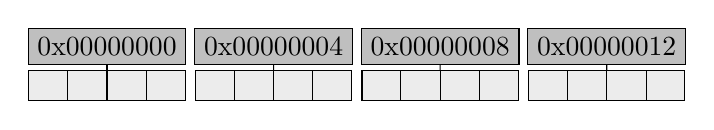
\begin{tikzpicture}[start chain, level distance=0.5cm, node distance=0.1cm, every on chain/.style={draw, fill=lightgray, minimum width=2cm}]
        \node [on chain] {0x00000000} child {node [cell] {}};
        \node [on chain] {0x00000004} child {node [cell] {}};
        \node [on chain] {0x00000008} child {node [cell] {}};
        \node [on chain] {0x00000012} child {node [cell] {}};
    \end{tikzpicture}
    \caption{Four word-sized memory cells in a 32-bit computer}
\end{figure}
\noindent
For instance, saving a 4 byte \textbf{int}
\tikz[baseline=-0.5ex]{%
    \node[cell, rectangle split part fill={green!50},] {};}
in our memory will result in the integer being properly aligned without doing any special work
because an int on this architecture is exactly 4 byte which will fit perfectly into the first slot.
\begin{figure}[H]
    \centering
    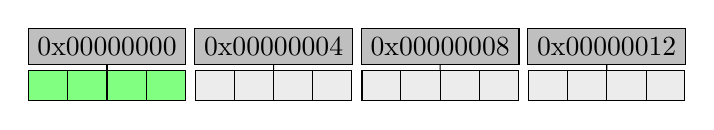
\begin{tikzpicture}[start chain, level distance=0.5cm, node distance=0.1cm, every on chain/.style={draw, fill=lightgray, minimum width=2cm}]
        \node [on chain] {0x00000000} child {node [cell, rectangle split part fill={green!50},] {}};
        \node [on chain] {0x00000004} child {node [cell] {}};
        \node [on chain] {0x00000008} child {node [cell] {}};
        \node [on chain] {0x00000012} child {node [cell] {}};
    \end{tikzpicture}
    \caption{Our memory with an int in it}
\end{figure}

\noindent
If we instead decided to put a \textbf{char}
\tikz[baseline=-0.5ex]{%
    \node[cell, rectangle split part fill={red!50,lightgray!30}] {};}
, a \textbf{short}
\tikz[baseline=-0.5ex]{%
    \node[cell, rectangle split part fill={blue!50,blue!50,lightgray!30}] {};}
and an \textbf{int}
\tikz[baseline=-0.5ex]{%
    \node[cell, rectangle split part fill={green!50},] {};}
into our memory we would get a problem if we did so na\"ively without worrying for alignment.
\begin{figure}[H]
    \centering
    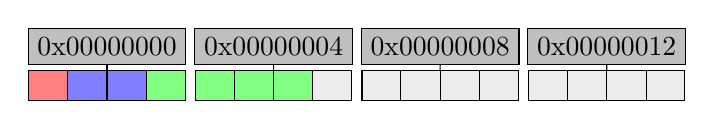
\begin{tikzpicture}[start chain, level distance=0.5cm, node distance=0.1cm, every on chain/.style={draw, fill=lightgray, minimum width=2cm}]
        \node [on chain] {0x00000000} child {node [cell, rectangle split part fill={red!50,blue!50,blue!50,green!50}] {}};
        \node [on chain] {0x00000004} child {node [cell, rectangle split part fill={green!50,green!50,green!50,lightgray!30}] {}};
        \node [on chain] {0x00000008} child {node [cell] {}};
        \node [on chain] {0x00000012} child {node [cell] {}};
    \end{tikzpicture}
    \caption{Misaligned memory}
\end{figure}

\noindent
This would need two memory accesses and some bitshifting to fetch the \textbf{int}. Effectively
that means it will take at least two times as long as it would if the data were properly aligned.
For this reason, computer scientists came up with the idea of adding padding
\tikz[baseline=-0.5ex]{\node[cell, rectangle split part fill={darkgray,lightgray!30},] {};}
to data in memory so
it would be properly aligned. In our example, adding padding after the first byte, the char, would
ensure that the last part of the data would be properly aligned in memory:

\begin{figure}[H]
    \centering
    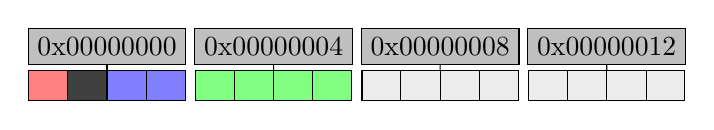
\begin{tikzpicture}[start chain, level distance=0.5cm, node distance=0.1cm, every on chain/.style={draw, fill=lightgray, minimum width=2cm}]
        \node [on chain] {0x00000000} child {node [cell, rectangle split part fill={red!50,darkgray,blue!50,blue!50}] {}};
        \node [on chain] {0x00000004} child {node [cell, rectangle split part fill={green!50}] {}};
        \node [on chain] {0x00000008} child {node [cell] {}};
        \node [on chain] {0x00000012} child {node [cell] {}};
    \end{tikzpicture}
    \caption{Properly aligned memory using padding}
    \label{tikz:struct1}
\end{figure}

\noindent
The figure above is considered \textbf{naturally aligned}. Compilers will automatically add
correct padding for the target platform unless this feature is deliberately switched off.

\subsection{Consequences of Misalignment}
The consequences of data structure misalignment vary widely between architectures. Some RISC, ARM
and MIPS processors will respond with an alignment fault if an attempt is made to access a
misaligned address. Specialized processors such as DSPs usually don't support accessing
misaligned locations. Most modern general purpose processors are capable of accessing misaligned addresses, albeit
at a steep performance hit of at least two times the aligned access time. Very modern x86\_64
processors are capable of handling misaligned accesses without a performance hit. SSE requires
data structures to be aligned per specification and would result in undefined behavior if
attempted to be used with unaligned data.

\section{Data Structure Alignment}
This chapter will introduce the reader to the alignment of simple real world \textbf{structs} in C.
It will use a series of examples to do so.
\subsection{Example With Structs}
The following struct reflects the struct in \autoref{tikz:struct1}.
\begin{listing}[H]
    \begin{minted}{c}
        struct Foo {
            char x; // 1 byte
            short y // 2 bytes
            int z; // 4 bytes
        };
    \end{minted}
    \caption{Example of a struct that needs padding}
\end{listing}
\noindent
This struct's na\"ive would be 1 byte + 2 bytes + 4 bytes = 7 bytes. The keen reader will know, of 
course, that it's actually going to be 8 bytes due to padding.

\begin{framed}
    A struct is always aligned to the largest type's alignment requirements
\end{framed}
\noindent
As we will see now, this can yield some rather inefficient structures:
\begin{listing}[H]
    \begin{minted}{c}
        struct Foo {
            char x; // 1 byte
            double y // 8 bytes
            char z; // 1 bytes
        };
    \end{minted}
    \caption{Example of an inefficient struct}
\end{listing}
The struct's naive size would be 1 byte + 8 bytes + 1 bytes = 10 bytes. However, its effective size is 24 byte!
\\
The memory ineffiency can be minimized by reordering the members like so:
\begin{listing}[H]
    \begin{minted}{c}
        struct Foo {
            char x; // 1 byte
            char z; // 1 bytes
            double y // 8 bytes
        };
    \end{minted}
    \caption{Example of how reordering a struct can make it more memory efficient}
\end{listing}
\noindent
Now it's only 16 bytes which is the best we can do if we want to keep our memory naturally aligned.

\subsection{Padding In The Real World}
The previous chapters might lead the reader to believe that a lot of manual care has to be taken
about data structures in C. In reality, however, it should be noted that just about every
modern compiler will automatically use data structure padding depending on architecture.
Some compilers even support the warning flag \verb|-Wpadded| which generates helpful warnings
about structure padding. These warnings help the programmer take manual care in case a more
efficient data structure layout is desired.
\begin{listing}[H]
    \begin{verbatim}
        clang -Wpadded -o example1 example1.c
        example1.c:5:11: warning: padding struct 
        'struct Foo' with 1 byte to align 'y' [-Wpadded]
        short y;
              ^
        1 warning generated.
    \end{verbatim}
    \caption{Example warning generated by clang using -Wpadded}
\end{listing}

If desired, it's actually possible to prevent the compiler from padding a struct using either
\verb|__attribute__((packed))| after a struct definition, \verb|#pragma pack (1)| in
front of a struct definition or \verb|-fpack-struct| as a compiler parameter. It's important to
note that using either of these will generate an incompatible ABI.
We can use the \verb|sizeof| operator to check the effective size of a struct and output it during
runtime using \verb|printf|.

\subsection{Performance Implications}
As with so many things in the real world where buying faster machines is usually a lot cheaper than
paying programmers, we have to ask ourselves whether worrying about memory alignment is even worth
it and whether we should worry about it at all. The resolve to that is that it depends, though most likely
we'll not have to think about it unless in special use cases like kernels, device drivers,
extremely memory limited computers or when using a really, really old compiler that is not good at
generating code for our architecture.

However, we should still know what kind of performance implications we are looking at before
disregarding the problem altogether. So let's look at the performance impact of misaligned memory.
For the benchmark, we'll be using two identical structs except for one difference: One of them is
aligned while the other is misaligned.
\begin{listing}[H]
    \begin{minted}{c}
        struct Foo {
            char x;
            short y;
            int z;
        };

        struct Foo foo;

        clock_gettime(CLOCK, &start);
        for (unsigned long i = 0; i < RUNS; ++i) {
             foo.z = 1;
             foo.z += 1;
        }
        clock_gettime(CLOCK, &end);
    \end{minted}
    \label{struct-bench-aligned}
    \caption{Aligned struct for the benchmark}
\end{listing}

\begin{listing}[H]
    \begin{minted}{c}
        struct Bar {
            char x;
            short y;
            int z;
        } __attribute__((packed));

        struct Bar bar;

        clock_gettime(CLOCK, &start);
        for (unsigned long i = 0; i < RUNS; ++i) {
             bar.z = 1;
             bar.z += 1;
        }
        clock_gettime(CLOCK, &end);
    \end{minted}
    \label{struct-bench-misaligned}
    \caption{Misaligned struct for the benchmark}
\end{listing}
\noindent
The benchmark was compiled with gcc (GCC) 4.8.2 20131219 (prerelease) using
\verb|gcc -DRUNS=400000000 -DCLOCK=CLOCK_MONOTONIC -std=gnu99 -O0| and run on an
Intel Core i7-2670QM CPU on Linux 3.12.5.
\\
Results:
\begin{tabular}{l|l}
    aligned runtime: & 9.504220399 s\\
    unaligned runtime: & 9.491816620 s
\end{tabular}

We can immediately see that both runs take about the same time. This behavior was already hinted at
by \cite{misaligned-data} which was referenced earlier. In modern Intel processors at least, there
is apparently no performance impact on misaligned memory accesses. Since these results are only
true on very modern processors, let's run this benchmark again on an older processor.
\\
\\
Rerunning the same benchmark on a Raspberry Pi with \(\frac 1 {10}\) the loop length and all
other variables being the same (kernel, compiler, flags) yields the following.
\\
Results:
\begin{tabular}{l|l}
    aligned runtime: & 12.174631568 s\\
    unaligned runtime: & 26.453561832 s
\end{tabular}

These results are a lot more on par with our expectations. In fact, the access times accurately
reflect our mind model of what should be happening: two memory accessess plus some bitshifting to 
extract the int.

\subsection{SSE}
Historically, when using SIMD instructions such as SSE, one was required to make sure the code
was aligned to 16 bytes boundaries per SSE specification. That means not only data structures
needed to be aligned to this boundary but also the stack itself. This was especially a problem when cross-compiling code for
32-bit platforms that were unaware of the fact that they should be aligned \cite{mingw-sse}. In a
later section, we will see what happens if a program making a library call has wrong assumptions
about byte alignment. However, mostly this just leads to crashes. Nowadays with x86\_64 being the
prevalent architecture for modern computers, this has become less of an issue since x86\_64
requires 16-byte alignment per default. This, however, was not the case on older 32-bit
architectures.

Even on 32-bit architectures most modern compilers automatically align to 16-byte boundaries when 
using SIMD types such as \verb|__m128|.
Even more modern compilers can automatically vectorize many types of loops and produce these types
(and therefore alignment) by themselves without the programmer explicitly telling the compiler to
do so, nor writing SIMD code for it. Due to that, programs might sometimes automatically be
16-byte aligned even when there is no obvious reason for that.

\section{Stack Alignment}
As hinted at by the previous section,different platforms make different assumptions about stack 
alignment. The reader should be informed about the major platforms in this regard:
\begin{itemize}
    \item Linux: depends (legacy is 4 byte, modern is 16 byte)
    \item Windows: 4 byte
    \item OSX: 16 byte
\end{itemize}
Knowing this is important because mixing stack alignment is very bad indeed!
\\
\\
Consider this:
\begin{listing}[H]
    \begin{minted}{c}
    void foo() {
        struct MyType bar;
    }
    \end{minted}
\end{listing}
This function and its struct look benign, yet what would happen if this were a function in a
library compiled with 16-byte alignment and code that assumed 4-byte alignment called it?
It would inevitably lead to \textbf{stack corruption} since the the stack pointer would either be
12 bytes too far or 12 bytes too short, depending on who calls whom.
\\
In the real world, this problem very rarely ever happens. If it happens, however, it's usually hard
to debug, especially if the programmer is not knowledgeable about this kind of problem. This issue 
only presents itself if we have cross-architecture calls that need special tricks such as
stack realignment. In gcc and clang, this can be accomplished by decorating a functiong with
\verb|__attribute__((force_align_arg_pointer))| or using \verb|-mstackrealign| as a compiler
argument to apply the decorator to every function. The reader should be aware, however, that this
has performance implications as this adds a realignment intro/outro routine to every function to
make sure the stack pointer comes back to where we expect it to be.

\section{Conclusion}
In conclusion, we've seen that modern compilers try to optimize data structures for maximum
performance using padding unless specified otherwise. This comes at the trade-off of bigger
structures in memory but given
the abundance of memory nowadays it seems negligible in comparison to the potential speedups this
optimization may have. We've also seen that even in case code is deliberately misaligned, modern
processors will still not take a hit, though older processors seem to be greatly affected by memory
misalignment.
\\
The only thing the programmer still needs to take manual care of is creating efficient data structures 
by ordering members so that memory waste by padding is minimized.

\bibliography{general}
\begin{thebibliography}{9}
    \bibitem{sse4}
        \url{http://software.intel.com/en-us/articles/increasing-memory-throughput-with-intel-streaming-simd-extensions-4-intel-sse4-streaming-load}

    \bibitem{misaligned-data}
        \url{http://www.agner.org/optimize/blog/read.php?i=142&v=t}

    \bibitem{mingw-sse}
        \url{http://www.peterstock.co.uk/games/mingw_sse/}
\end{thebibliography}

\end{document}
